\chapter{Implementation}

\section{The RTPS Library}

In this section we discuss the various classes which make up the Real-Time
Particle System framework. Filenames will be denoted as such \verb|rtpslib/RTPS.h|
and refer to the directory structure of the code \ref{appendix:code}.



\subsection{RTPS}

The entry point into the framework is the \verb|rtpslib/RTPS.h| header file. This file defines
the RTPS class which a user of the library will instanciate in order to run a
particle based simulation. The Application Programmers Interface (API) is
relatively simple, giving the user an object which only exposes two methods, a
\verb|update| function and an \verb|render| function. These two functions abstract
internal logic for updating the simulation and displaying of the particles. The
constructor to the class accepts either no arguments or an \verb|RTPSettings| object.
This object contains many settings including the type of simulation to
instanciate, rendering options as well as simulation parameters. 

The typical use case (with default settings) is envisioned as follows
\begin{cppcode}{0}
#include "RTPS.h"
using namespace rtps;
//... initialization phase ...
RTPSettings settings();
RTPS ps(settings);

//... run loop ...
while(true)
{
    //... event handling and game logic
    ps.update()
    //... rendering phase
    ps.render()
}

\end{cppcode}

The class is implemented in \verb|rtpslib/RTPS.cpp|.

\subsection{RTPSettings}

Options and parameters for the system are stored in a private STL Map object
defined in \verb|rtpslib/RTPSettings.h| and accessed through public getter and
setter methods. The available settings are not determined by this class, but by
the implementation of each system. This is desirable since different systems
will offer different combinations of settings and rather than creating,
implementing and innevitably changing new constructors, the proper combination
of settings can be set with calls to the setter functions. This is especially
convenient when developing for a user interface such as in Blender where the
configuration of settings is not known until runtime.  
An example of specifying the available settings for SPH can be found in
\verb|rtpslib/system/SPHSettings.h|.


An example of setting an option with an RTPSettings instance:
\begin{cppcode}{0}
settings->SetSetting("sub_intervals", 1);
\end{cppcode}

An example of getting an option with an RTPSettings instance:
\begin{cppcode}{0}
int sub_intervals =  settings->GetSettingAs<float>("sub_intervals");
\end{cppcode}

\subsection{System}

Interaction with the simulation is provided through the \verb|system| object which
will have various methods depending on what type of simulation was set in the
settings. The most important methods are those which allow the user to add
particles to a system, namely \verb|addBox|, \verb|addBall| and \verb|addHose|. For the fluid
simulation there is also the \verb|loadTriangles| method which allows the user to
pass in triangles for the fluid particles to collide with.

These methods are declared in the System.h header file which defines an
Abstract Class \verb|System|. The methods are implemented in the specific system
classes such as \verb|SPH| and \verb|Simple|.

\subsection{Common Structures}

Utilized throughout the code is the \verb|float4| struct. \verb|float4| structs are used
to represent coordinate positions of the particles, as well as many of the
properties associated with the particles such as density, velocity and force.
The functionality of the \verb|float4| class match the OpenCL \verb|float4| type as close
as possible. We have overloaded several operators for constructing and doing
arithmetic as well as provided a print function. This functionality allows the
developer to quickly construct data for interacting with the system. Being able
to reimplement an OpenCL routine on the CPU is also convenient for debugging
logic since it makes printing output much simpler. 
There is also the \verb|int4| struct which is similarly a vector of four integers
for more convenient communication with OpenCL.
the declarations and definitions for these structures and related functions can
be found in \verb|rtpslib/structs.h| and \verb|rtpslib/structs.cpp|


\subsection{Domain}

The \verb|Domain| class calculates and stores the parameters for a regular grid
on the interior of a cube. The cube serves as a bounding domain for the
particles in a simulation, wheras the grid is used to accelerate the neighbor
search for particles. It is important to note that the grid is not stored as a
set of nodes or cells, only the minimum and maximum of the cube along with the
size and number of cells in each dimension.

The \verb|Domain| class is found in \verb|rtps/domain/Domain.h| and
\verb|rtps/domain/Domain.cpp| alongside \verb|rtps/domain/IV.h| and
\verb|rtps/domain/IV.cpp| which define several helper functions for inserting
particles at regularly spaced intervals based on grid parameters.


\section{Nearest Neighbor Search}
The Nearest Neighbor Search (NNS) is essential to the SPH simulation because it
allows for the efficient updating of a particle's forces based on surrounding
particles. The NNS is implemented in two distinct phases, preparation and
lookup. The preparation phase prepares the data structures needed at the
beginning of each update, while the lookup phase is performed by any routine
which needs access to nearest neighbors.

\subsection{Preparation}
The first step in the NNS preparation is creating an integer hash value for
each particle to be sorted. This hash value is created by overlaying a uniform
grid on the domain, calculating the cell which contains the particle and then
calculating a one dimensional index from the three-dimensional cell index.\cite{Krog2010}

\subsubsection{Hash}
The cell index is calculated as follows:
\begin{cppcode}{0}
int4 cell_index = (pos - grid_min) * grid_delta;
\end{cppcode}

Where \verb|grid_min| is a \verb|float4| representing the minimum coordinate of
the grid, obtained from the domain. \verb|grid_delta| is a \verb|float4|
containing the width of the cell in each dimension. The width of the cells is
calculated as twice the smoothing length of a particle. In this way a particle
will only be able to interact with particles in the 26 surrounding cells.


The hash is calculated as follows:
\begin{cppcode}{0}
int gx = cell_index.x
int gy = cell_index.y
int gz = cell_index.z
int hash = (gz*grid_res.y + gy) * grid_res.x + gx;
\end{cppcode}

Where \verb|grid_res| is an \verb|int4| containing the number of cells in each dimension.


The hash for each particle is stored in an integer array by the \verb|Hash|
class defined in \verb|rtpslib/system/common/Hash.cpp| with the OpenCL kernel
implemented in \\ \verb|rtpslib/system/common/cl_src/hash.cl|

\subsubsection{Sort}
The hash array is then sorted using the Bitonic Sort implementation provided by
NVIDIA\cite{NVBitonic}. The C interface to the OpenCL code was replaced with a
C++ interface defined in \verb|rtpslib/system/common/BitonicSort.cpp|. The
Bitonic Sort implementation can only operate on arrays or subsets of arrays
with power of two lengths, so the sort always operates on the number of
particles rounded up to the nearest power of two. The sort is performed on the
hash values of each particle, with an array of indices being permuted along
with the hashes.

\subsubsection{Permute}
Once the hash and indices array are sorted, the arrays for particle position,
velocity, veleval and color are permuted according to the reordered index
array. This leaves all the particles and their associated values sorted
according to their spatial position. The \verb|Permute| class is defined in
\verb|rtpslib/system/common/Permute.cpp| with the OpenCL Kernel implemented in
\verb|rtpslib/system/common/cl_src/permute.cl|.


\subsubsection{Cell Indices}
The next step in the preparation is to update two arrays which keep track of
which cells are populated with particles. These two arrays are
\verb|cell_indices_start| and \verb|cell_indices_end|, where the former has a
value of -1 if no particles are present in the cell, or the index into the
particle array of the first particle in the cell. The latter contains the index
into the particle array of the last particle contained in a cell.
The \verb|CellIndices| class is defined in
\verb|rtpslib/system/common/CellIndices.cpp| with the OpenCL Kernel implemented in
\verb|rtpslib/system/common/cl_src/cellindices.cl|.


The \verb|cellindices| kernel utilizes local memory to decrease global memory
accesses in the process of setting the \verb|cell_indices| arrays. 
The C++ code allocates a local memory array equal to the workgroup size plus 1.
This array is populated by the current particles hash and then the first thread
sets the first element of the array to the hash of the previous particle.
\begin{cppcode}{0}
uint tid = get_local_id(0);
sharedHash[tid+1] = hash; 

if (index > 0 && tid == 0)
{   
    // first thread in block must load previous particle hash
    uint hashm1 = sort_hashes[index-1] < ncells ? sort_hashes[index-1] : ncells;
    sharedHash[0] = hashm1;
}
\end{cppcode}

The kernel waits for all threads to finish this computation with a memory fence:
\begin{cppcode}{0}
barrier(CLK_LOCAL_MEM_FENCE);
\end{cppcode}

The accelerated part of the cell index assignment is given here:
\begin{cppcode}{0}
if (index > 0)
{
    if(sharedHash[tid] != hash)
    {
        cell_indices_start[hash] = index;
        cell_indices_end[sharedHash[tid]] = index;
    }
}
\end{cppcode}

This will update the appropriate start and end indices if the hash between
neighboring particles is different.

\subsection{Lookup}
A neighbor lookup is performed by calculating the grid cell of a particle and
iterating over all of the particles in that cell and its 26 neighbors. The grid
cell and corresponding hash are calculated with the same routines used in the
preparation. The neighbor search is composed of three functions, the first two
found in \verb|rtpslib/system/sph/cl_src/cl_neighbors.h| and the last found in
the \verb|Force| and \verb|Density| kernels.

\subsubsection{IterateParticlesInNearbyCells}
This function loops over the 26 cells neighboring the cell of the particle
being queried. For each cell it calls the IterateParticlesInCell function.

\subsubsection{IterateParticlesInCells}
This function first determines the start index into the particle array from the
current cell's hash and the \verb|cell_indices_start| array. If the value is
not $-1$ then the end index is obtained from the \verb|cell_indices_end| array.
If the hash of the cell is greater than the maximum hash size the routine exits
early to avoid accessing non-existant array elements. The routine then iterates
over all of the particles from the start index to the end index and calls the
ForNeighbor function.

\subsubsection{ForNeighbor}
This function now has access to the original particle being queried as well as
the index of a neighboring particle. The code for the previous two routines is
contained in a header file which is included by the kernel which implements the
ForNeighbor function. This allows for kernels with different functionality to
reuse the neighbor search code. Different kernels may require access to
different arrays within the ForNeighbor routine, in order to pass different
arguments through all three routines \verb|#define| macros are used to specify
the arguements of each function and the values passed through. An example of
this is provided in Appendix \ref{appendix:density}.

\section{Particle Insertion and Deletion}
Particles can be dynamically inserted into and deleted from the simulation by
taking advantage of the hashing and sorting functionality. The number of
particles in the system is kept track of by the \verb|SPH| instance.
Calculations in the simulation are only done on the first $num$ elements of the
relevant arrays (such as position, velocity, force etc.) where $num$ is the
current number of particles. The values in the position array for indices
greater than $num$ is set to a location that will always place them outside of
the grid (e.g. a positive multiple of the grid max). Any particle outside of
the grid will receive a hash value greater than the maximum hash value, thus
when the particle array is sorted, the active particles are always first in the
array. 

\subsection{Insertion}
Particles are inserted by setting the values of the position, velocity and
color arrays immediately after the $num$ index and incrementing $num$ by the
number of particles added. When the particles are sorted, the new particle
positions will be inside the grid and will be part of the new $num$ of
particles to be used in the simulation.

\subsection{Deletion}
Deletion of particles is accomplished by moving particles outside of the grid.
When the \verb|Hash| kernel calculates the hash for a particle which falls
outside of the grid it assigns the maximum hash value to that particle.
The $num$ of active particles is updated by taking advantage of the
\verb|CellIndices| kernel. The value of the element at the maximum hash value
of the \verb|cell_indices_start| after the \verb|CellIndices| kernel execution
gives the start index of the particles outside the grid and conversly the
number of particles which are inside the grid. The number of particles is then
set to this value and the deleted particles are no longer used in the
simulation.

\section{Parameters}
Two structures are defined which hold the all of the parameters for the system,
one is the \verb|GridParams| structure which holds all the parameters relevant
to the Domain and spatial grid while the other is \verb|SPHParams| which holds
all of the parameters relevant to the SPH simulation. These structures are
populated by the \verb|SPH| and \verb|SPHSettings| classes and passed to all of
the OpenCL kernels as constant memory structures. The \verb|SPHParams|
structure is listed in Appendix \ref{appendix:sphparams}.


\subsection{Calculated Parameters}
A subset of the physical and simulation parameters are automatically calculated
based on one user defined parameter, the maximum number of particles. The
per-particle volume is calculated by dividing a set volume by the maximum
number of particles. 
\begin{cppcode}{0}
float VP = 2 * .0262144 / max_num;              //Particle Volume [ m^3 ]
\end{cppcode}

The mass of each particle is the product of the rest density and the particle volume.
\begin{cppcode}{0}
float mass = 1000. * VP;                         //Particle Mass [ kg ]
\end{cppcode}

The rest distance between particles is a fraction of the particle radius.
\begin{cppcode}{0}
float rest_distance = .87 * pow(VP, 1.f/3.f);   //rest distance between particles [ m ]
\end{cppcode}

The smoothing distance is simply twice the rest distance.
\begin{cppcode}{0}
float smoothing_distance = 2.0f * rest_distance; //interaction radius
\end{cppcode}

The simulation is scaled to the coordinate space of the user specified Domain
by relating the volumes of each particle to the volume of the Domain.
\begin{cppcode}{0}
float domain_vol = (dmax.x - dmin.x) * (dmax.y - dmin.y) * (dmax.z - dmin.z);
float simulation_scale = pow(.5f * VP * max_num / domain_vol, 1.f/3.f);
\end{cppcode}

These calculations are specified in \verb|rtpslib/system/SPHSettings.cpp|.


\section{SPH Force Calculations}
The force calculations defined by the SPH formulation are implemented in three
distince phases, density, force and collision.

\subsection{Density}
The density of each particle is calculated by the summation over its neighbors
as given by the SPH formulation. The density calculation only depends on the
position of the particles and the particle mass. In this implementation the
particle mass is uniform for all particles and is thus passed in as a constant.
The density calculation is controlled by the \verb|Density| class defined in
\verb|rtpslib/system/sph/Density.cpp| and the OpenCL kernel is defined in
\verb|rtpslib/system/sph/cl_src/density.cl|. The density kernel is included in
Appendix X.

\subsection{Force}
The force calculation is controlled by the \verb|Force| class defined in
\verb|rtpslib/system/sph/Force.cpp| and the OpenCL kernel is defined in
\verb|rtpslib/system/sph/cl_src/force.cl|. 


The forces according to the pressure and viscosity terms of the SPH formulation
are calculated as well as a smoothing factor known as XSPH.\cite{Krog} The XSPH
calculation is given as follows:

\begin{cppcode}{0}
    float Wijpol6 = Wpoly6(r, sphp->smoothing_distance, sphp);
    float4 xsph = 2.f * sphp->mass * Wijpol6 * (velj-veli)/(di+dj);
    xsph += xsph * (float)iej;
\end{cppcode}

Where \verb|veli| and \verb|velj| are the velocities at particles i and j
respectively and \verb|di| and \verb|dj| are the densities at particles i and j
respectively. The value of iej is given by:

\begin{cppcode}{0}
int iej = index_i != index_j;
\end{cppcode}

Which is used to nullify any force or XSPH contributions from a particle with
itself. Additional care must be taken for particles which obtain the same
position since the calculation of the $W_{spiky}$ kernel derivative involves
the division of the distance between particles. A divide-by-zero error is
avoided by setting the distance used in the kernel to the maximum between the
distance and a small epsilon, $10^{-6}$.


\subsection{Collision}
The routines which calculate the repulsion force contributions
from collisions are specified in the
\verb|rtpslib/system/sph/cl_src/cl_collision.h| header file.

Collisions with the boundary are computed by the kernel in
\\ \verb|rtpslib/system/sph/cl_src/collision_wall.cl| and controlled by the
\verb|CollisionWall| class in \verb|rtpslib/system/sph/Collision_wall.cpp|.
A collision with the boundary is determined by a simple distance query. The
collision test with the bottom of the domain is given as an example: 
\begin{cppcode}{0}
float diff = sphp->boundary_distance - (p.z - gp->bnd_min.z);
if (diff > sphp->EPSILON)
{
    float4 normal = (float4)(0.0f, 0.0f, 1.0f, 0.0f);
    force += calculateRepulsionForce(normal, v, sphp->boundary_stiffness, 
            sphp->boundary_dampening, diff);
}
\end{cppcode}

Here $p$ is the particle position, $v$ is the particle velocity and
\verb|gp->bnd_min.z| is the Z coordinate of the bottom of the domain.
\\

Collisions with triangles are computed by the \verb|collision_triangle| kernel in
\\ \verb|rtpslib/system/sph/cl_src/collision_tri.cl| and controlled by the
\verb|CollisionTriangle| class in \verb|rtpslib/system/sph/Collision_triangle.cpp|.

Triangles are defined by their three vertices and a normal in a \verb|Triangle| structure:
\begin{cppcode}{0}
typedef struct Triangle
{
    float4 verts[3];
    float4 normal;
} Triangle;
\end{cppcode}

The triangles are stored in a vector of \verb|Triangle| structures in C++ and
passed to OpenCL as an array. The \verb|collision_triangle| kernel is executed
with one thread per-particle. The first thread in each workgroup copies a section of the
triangle array into local memory. After synchronizing the threads with a local
barrier, each thread iterates over the list of triangles and determines
particle-triangle collisions with a ray-triangle intersection
test.\cite{Ericson} If a collision is detected the force on a particle is
modified according to the repulsion force formula. Once all of the triangles in
the section have been iterated over, the next section of triangles is copied to
local memory and iterated over. This process is repeated until all of the
triangles have been checked for collisions.


\section{Integration}

Integration of the forces and velocities of the particles are computed by the
\verb|leapfrog| kernel in \verb|rtpslib/system/sph/cl_src/leapfrog.cl| and
controlled by the \verb|LeapFrog| class in
\verb|rtplslib/system/sph/LeapFrog.cpp|.

In the following code snippets, the following variables will be referred to:
$p$ is the position of a particle, $v$ is the velocity and $f$ is the force.


Gravity is first added to the Z component of force of each particle. The
magnitude of the force is scaled to a maximum speed given by a the \verb|velocity_limit| parameter:
\begin{cppcode}{0}
float speed = length(f);
if (speed > sphp->velocity_limit) 
{
    f *= sphp->velocity_limit/speed;
}
\end{cppcode}

The force is then integrated to update the velocity. The velocity is
effectively smoothed by the XSPH calculated in the \verb|force| kernel adjusted
by a user defined parameter. The position is then updated by integrating the
velocity.
\begin{cppcode}{0}
float4 vnext = v + dt*f;
vnext += sphp->xsph_factor * xsph_s[i];
p += dt * vnext;
\end{cppcode}

The LeapFrog integration is calculated and stored for use in the force and XSPH
calculations in the \verb|force| kernel.
\begin{cppcode}{0}
float4 veval = 0.5f*(v+vnext);
\end{cppcode}




\section{OpenCL}

The framework provides several classes to abstract access to OpenCL routines.
The underlying OpenCL functionality is provided by the Khronos C++ header
files.\cite{OpenCL} 

The purpose of RTPS OpenCL classes is convenience for the developer, hiding tedious
and repetitive behavior and providing sensible default behavior. The classes
are not intended to be a general replacement for the official OpenCL interface,
and focus primarily on the functionality required in this project.

\subsection{CLL}
The fundamental OpenCL class provided by the library is the \verb|CLL| class
defined in \verb|rtpslib/opencl/CLL.cpp|. When this class is instanciated it
creates and stores the OpenCL context and command queue to be used by the
\verb|RTPS| and \verb|System| classes. The class also provides routines for
building programs and loading kernels.

\subsection{Kernel}
The \verb|Kernel| class abstracts the creation and use of OpenCL kernels.
Instanciating a \verb|Kernel| class will load a kernel from source using the
context from the provided \verb|CLL| instance. The primary purpose of this
class is to abstract kernel execution, simplifying the process of setting
kernel arguements, automating the timing of kernel executions and hiding the
command queue syntax.


The \verb|Kernel| class is defined in \verb|rtpslib/opencl/Kernel.cpp|.


\subsection{Buffer}

The \verb|Buffer| class abstracts the creation and use of OpenCL buffers.
Buffers can be created from OpenGL vertex buffer objects or STL vectors.
Convenience methods are provided for copying data to and from the GPU.

The extent of the simplification can be seen by comparing the code for copying a
standard vector to the GPU with the Krhonos C++ API
\begin{cppcode}{0}
     std::vector<float> a; 
     ... //initialize a 
     err = queue.enqueueWriteBuffer(cl_a, CL_TRUE, 0, array_size, &a[0], NULL, 
         &event);
\end{cppcode}

with the utility classes provided by this project
\begin{cppcode}{0}
    std::vector<float> a; 
     ... //initialize a 
    cl_a.copyToDevice(a);
\end{cppcode}


The \verb|Buffer| class is defined in \verb|rtpslib/opencl/Buffer.cpp|.


\subsection{CL/GL Interoperability}
A key performance consideration with GPU computing is memory transfer, as
discussed there is a large difference in speed between $local$ and $global$
memory, there is an even larger difference in the cost for transfering memory
between the host (CPU) memory and the device (GPU). Due to this cost it is
desirable to perform as many operations as possible on the GPU without needing
to transfer data between the host and the device.


As such a key feature in OpenCL programming for games is the ability to share a
context with OpenGL, allowing OpenCL to directly access and manipulate OpenGL
memory objects. With this feature one can avoid any transfer of data associated
with the graphics of the application, therefor if the computation done in
OpenCL changes the positions of objects to be rendered in OpenGL, it is all
done in the same memory location.



\subsection{Issues}
In the course of developing this project several small issues have been raised
whos solutions were not trivial. This section describes those issues and the
design decisions made to address them.

\subsubsection{Kernel Compilation Caching}
OpenCL is designed to compile kernels at runtime, and once those kernels are
compiled the binary version is cached for the context in which it is run. This
cuts down on the cost of running a kernel after the first compilation. An issue
arises with the Apple implementation of OpenCL when using include directives in
OpenCL code. If a kernel has been executed and cached by the Apple runtime,
changes to files included in the kernel will not be reflected in the following
run, indicating that the cache is not updated. Included files (such as header
files) are often used for isolating functionality which is common to many
routines, and it is desirable to develope this functionality in one place and
have all the code which uses it updated at once. With the caching issue this
style of development was not possible. The solution put forth in this project
was to use the g++ preprocessor to preprocess the OpenCL files after making
changes to the headers. This would generate OpenCL source files which had
everything in one file so that the kernel which OpenCL was caching was forced
to update. 


\subsubsection{float4}
The OpenCL 1.0 specification defines the \verb|float4| type as a vector of four
floating point numbers. Since the simulation in this project is designed to be
3 dimensional it is the most convenient data type for storing arrays of
coordinates. The OpenCL 1.1 standard does define a \verb|float3| type, but as
of this writing the 1.0 standard is still the most widely available
implementation so we use \verb|float4| for backwards compatibility. It is also
convenient to package many variables into a single array for use on the GPU,
and as such one may utilize the unused components of 3 dimensional vectors for
storing some scalar values.

\subsubsection{GL Context Sharing on the Mac}
The Apple implementation of OpenCL uses a specific extension for OpenGL context
sharing which requires a specific way of creating an OpenCL context. The C++
headers provided by Khronos did not allow for this manner of Context creation,
leading to the following modification of $cl.hpp$ provided by Khronos
\begin{cppcode}{1448}
Context(cl_context_properties* properties, cl_int* err = NULL)
    {    
        cl_int error;
        object_ = ::clCreateContext(
            properties, 0, 
            0,   
            NULL, NULL, &error);

        detail::errHandler(error, __CREATE_CONTEXT_FROM_TYPE_ERR);
        if (err != NULL) {
            *err = error;
        }    

    }    
\end{cppcode}

\subsection{Timing}

When developing a performance critical application it is important to know how
much time subroutines are taking to execute. OpenCL provides a mechanism for
timing the execution time of a kernel on the GPU, which is essential since
kernels may be executed asynchronously from the command queue. As part of the
convenience classes provided by this project for OpenCL, executing a kernel
automatically times its execution and returns the time in milliseconds.




\subsection{Debugging Routines}

It is often desirable to output the values of a variable while debugging code,
however this is currently not simple with OpenCL. We have implemented a pattern
using a set of macros in the kernel source code as well as two dedicated arrays
with corresponding GPU buffers. When debugging a kernel the programmer will
pass the two buffers as the final arguments, with the first buffer being an
array of \verb|float| and the second buffer being an array of \verb|int4|. 
Inside the kernel the user will have the folowing macros defined (we include
these in our cl\_macros.h header)
\begin{cppcode}{0}
#define DEBUG_ARGS  , __global float4* clf, __global int4* cli
#define DEBUG_ARGV  , clf, cli
\end{cppcode}

Here \verb|DEBUG_ARGS| is added to the kernel's list of parameters as well as
to the argument list of any functions which we wish to debug in.
\verb|DEBUG_ARGV| is used when calling functions with the debug arguments. This
way one can easily extend or change the debugging arrays without the tedious
task of adding and subtracting arguments to kernel and function definitions,
and when done debuging one can simply redefine the macros to be empty.

Once the programmer has these arrays available inside of the kernel and updates
their contents in OpenCL, the next step is bringing these arrays back to the
CPU for printing and other analysis. The \verb|Buffer| class provides a
\verb|copyToHost| routine which makes this straight forward. Simply initialize
an empty vector of the same type as the array, with size equal to the
number of elements to be copied from the GPU. Then pass this vector to the routine:
\begin{cppcode}{0}
//where mybuffer was instantiated like Buffer<float4>(...)
std::vector<float4> tmp(100);
mybuffer.copyToHost(tmp);
//or to copy 100 elements starting at the 500th element (offset of 500)
mybuffer.copyToHost(tmp, 500);
\end{cppcode}

The vector \verb|tmp| will then be populated with the data from the GPU and can
be printed and manipulated using all of the familiar CPU functions available to
the programmer. 

\section{CMake}
CMake is a cross-platform, open-source build system.\cite{CMake} CMake
abstracts the process of generating Makefiles for the compilation of large
projects. This abstraction handles the differences between operating systems
and compilation toolchains. CMake is used in this project to compile and link
the library as well as standalone test applications. By using CMake the project
can be compiled with relative ease on Windows, Linux and Mac OS X.


CMake is also used by the Blender project as one of the supported build systems
for compiling the Blender software. This was a strong motivation behind using
CMake for the RTPS library. Since both projects use CMake it is relatively
straightforward to integrate the two. This is accomplished by placing the RTPS
library in a subdirectory of the Blender source tree and changing the Blender
$CMakelists.txt$ file to add the subdirectory. With this configuration
compiling Blender will also compile the RTPS library. By adding a few more
modifications to the Blender CMake configurations RTPS could be included and
linked against in Blender source code.



\section{OpenGL}

Rendering of the simulation is controlled by the \verb|Render| class or one of
its subclasses. The \verb|Render| class provides basic OpenGL rendering
functionality through the use of \verb|Vertex Buffer Objects| (VBO), which are OpenGL
Buffer types for storing coordinate based information. With the use of
OpenCL/OpenGL context sharing the positions of particles and their associated
color can be stored in a VBO and manipulated as OpenCL buffers without copying
or transfering data. The \verb|Render| class is passed in the OpenGL address
for the position and color VBOs as well as the RTPS settings object which
contains settings related to the rendering. The Render class is defined in
\verb|rtpslib/render/Render.h|.


\subsection{Points}
The most basic form of rendering provided simply displays each particle as a
filled in circle with a fixed radius. This rendering allows the developer to
see the behavior of the fluid with minimal overhead. The rendering is
accomplished using the OpenGL function $glDrawArrays$ with the \verb|GL_POINTS|
option and specifying the position and color VBOs with $glVertexPointer$ and
$glColorPointer$ respectively. The Point rendering functionality is implemented
in \verb|rtpslib/render/Render.cpp|

\begin{figure}[!htc]
 		\centering
		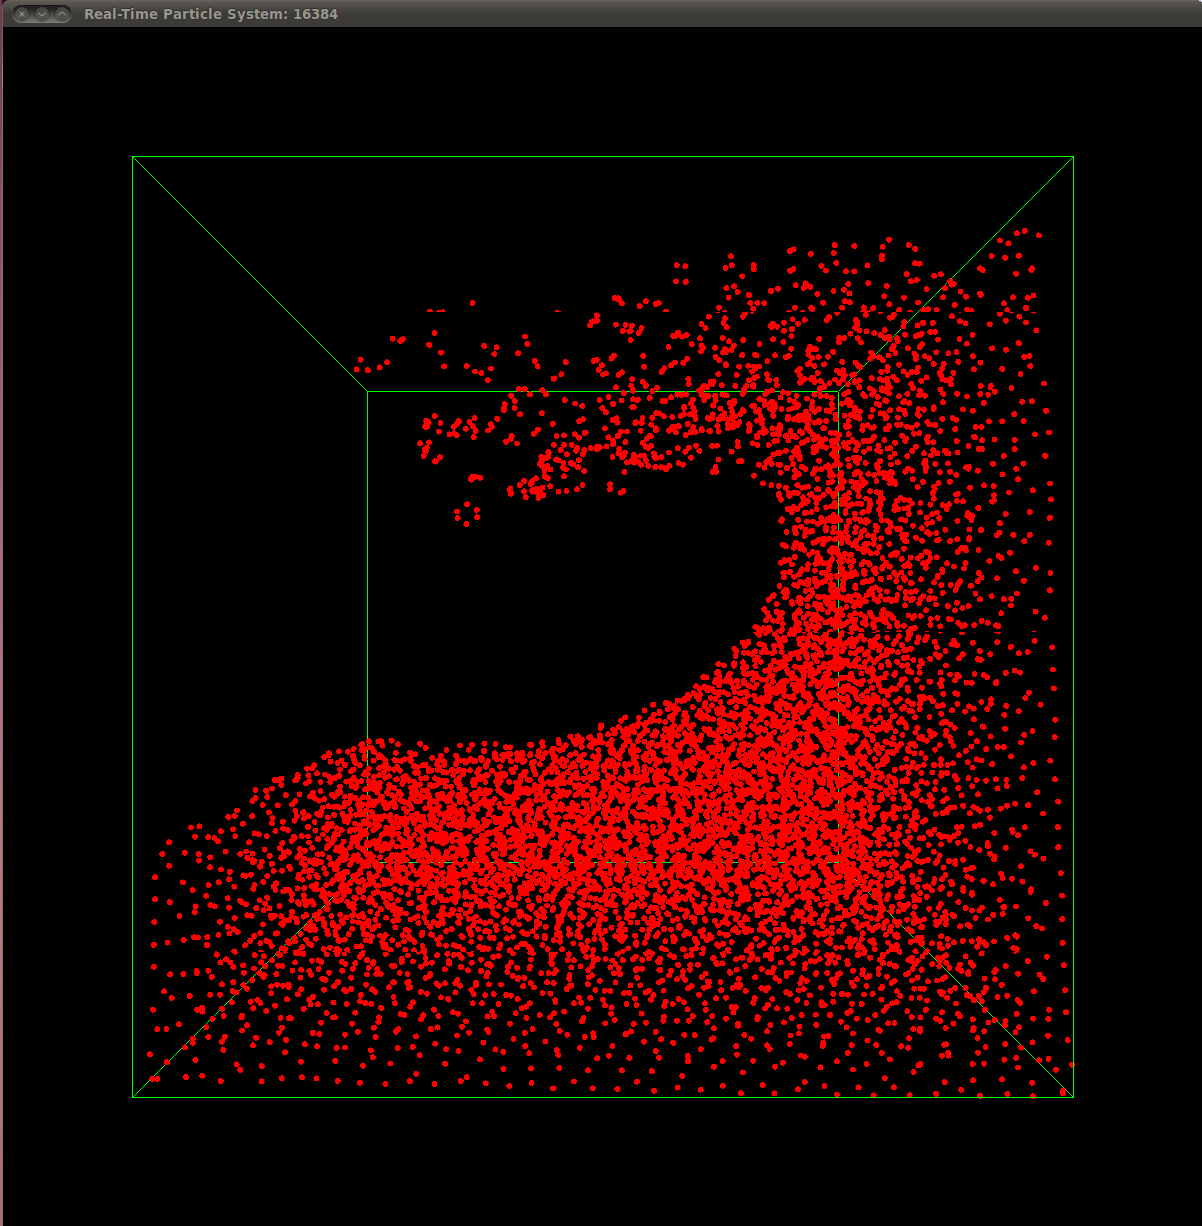
\includegraphics[scale=0.2]{figures/standalone.png}
        \caption{ Fluid rendered as Points in standalone application }
		\label{fig:points}
\end{figure}



\subsection{Point Sprites}
A common way to render particles is with a technique known as $billboarding$.
In this technique a small texture is rendered to a quad which is always aligned
to be perpendicular with the camera. With this technique it is possible to
improve upon the point rendering as well as fake some volumetric effects with
low computation cost.

\begin{figure}[!htc]
 		\centering
		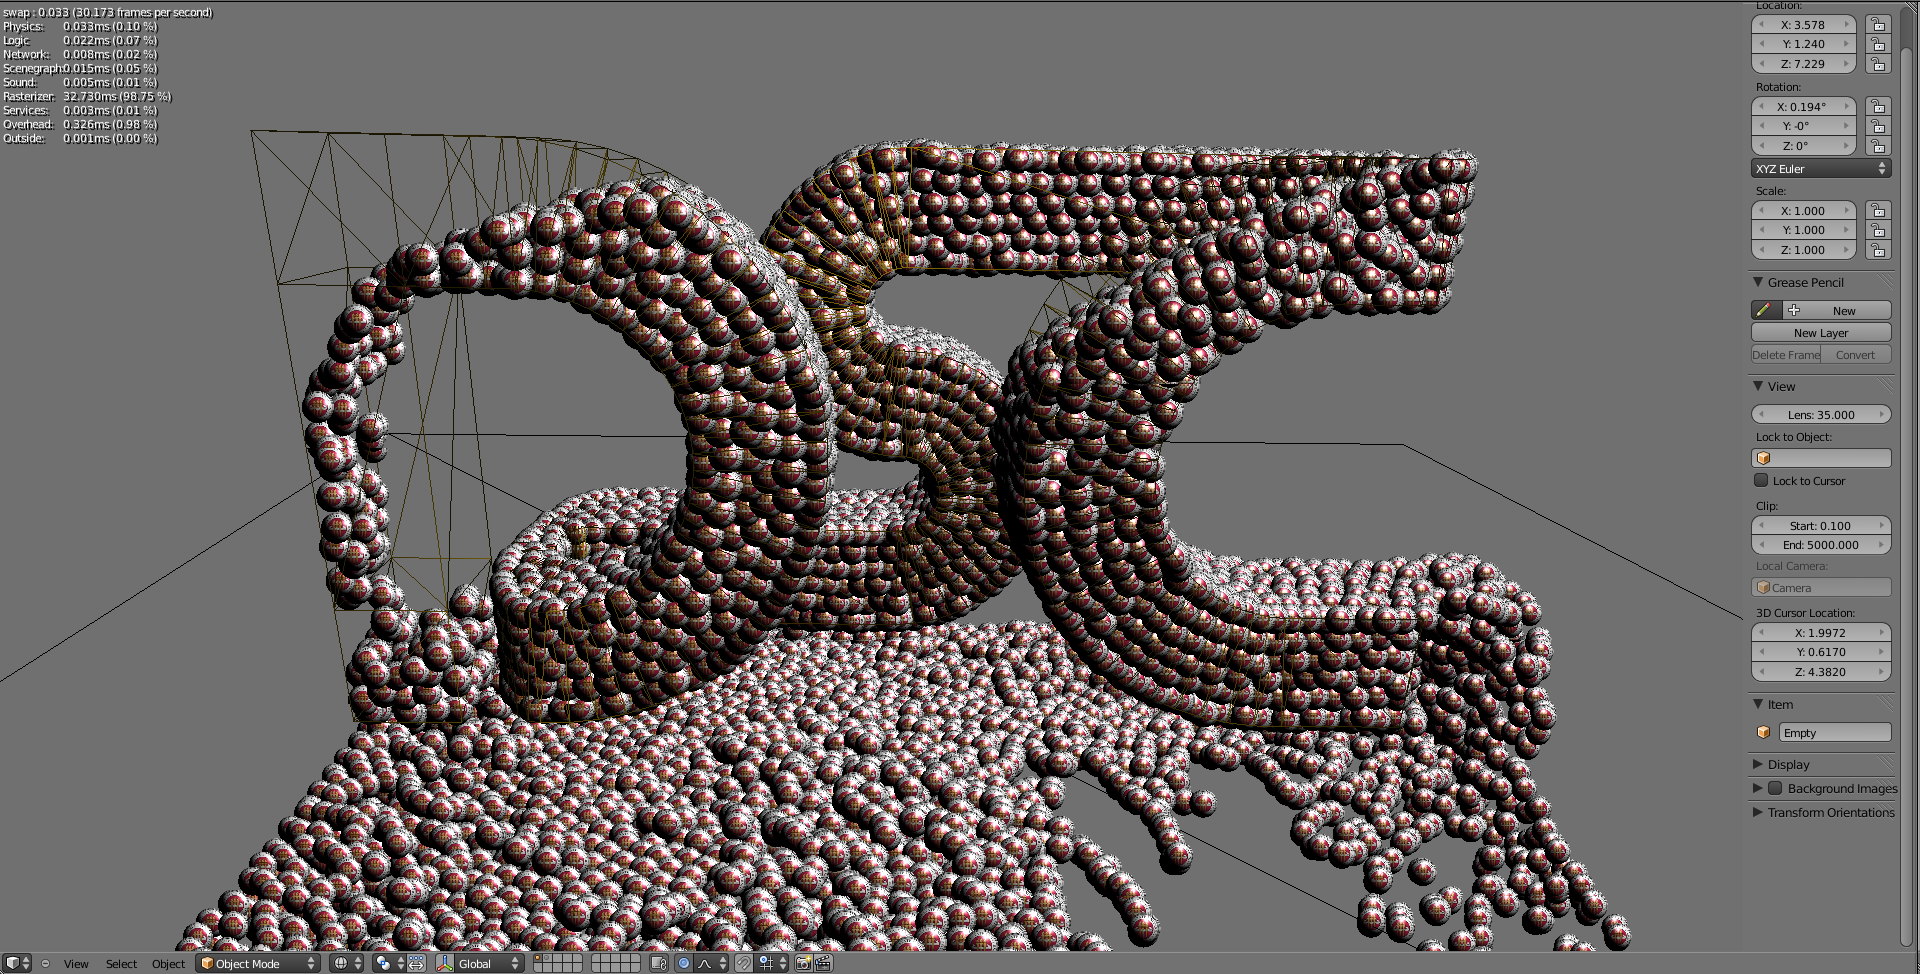
\includegraphics[scale=0.2]{figures/pointsprites.png}
        \caption{ Fluid rendered as PointSprites in Blender }
		\label{fig:pointsprites}
\end{figure}


The \verb|SpriteRender| class implements billboarding using the
\verb|GL_POINT_SPRITE| functionality in OpenGL which will create a textured quad
of a specified size centered at each coordinate in the position VBO. GLSL
vertex and fragment shaders are used to manipulate the appearance of the point
sprites. The default shaders use artificial lighting to fake the appearance of
spheres. Another set of shaders is provided in the code for loading of an image
for use as a texture on the billboards. The \verb|SpriteRender| class inherits
from \verb|Render| and overrides the $render$ function. The class is
implemented in \verb|rtpslib/render/SpriteRender.cpp| and the shaders are in
\verb|rtpslib/render/shaders|.


\section{Blender Source Modification}

In order to use the RTPS library inside the Blender Game Engine the source code
for Blender must be modified. The manner in which RTPS is exposed to Blender is
through a construct known as a Modifier. The purpose of a Blender Modifier is
to enable custom functionality on a Blender Object, usually resulting in a
modification of the Object's data. In the Blender Game Engine all modifiers on an Object are
$Applied$ at the start of a game and are $Updated$ every frame. The definition
of $Apply$ and $Update$ depend on the Modifier, and in the case of RTPS it is
desirable to instanciate the particle system when the Modifier is $Applied$ and
to calculate the next timestep when $Updated$.


Blender Modifiers are specified using the Blender DNA system, using a C
structure to store associated data. A Modifier's data can be exposed to the Blender User Interface
through Blender's Data API and Python scripting interface. The Blender Data API
is a way to programmatically access data structures used by Blender without
needing to know the details of how they are stored.\cite{b3dDataAPI} The User
Interface for Blender is controlled with Python, and the Python/RNA API gives
access to the Data API so that the values and functionality of a data structure
can be manipulated in the User Interface.\footnote{More information on
Blender's internal architecture is available at
\url{http://www.blender.org/development/architecture/}}


\subsection{User Interface}
%screenshot
\begin{figure}[!htc]
 		\centering
		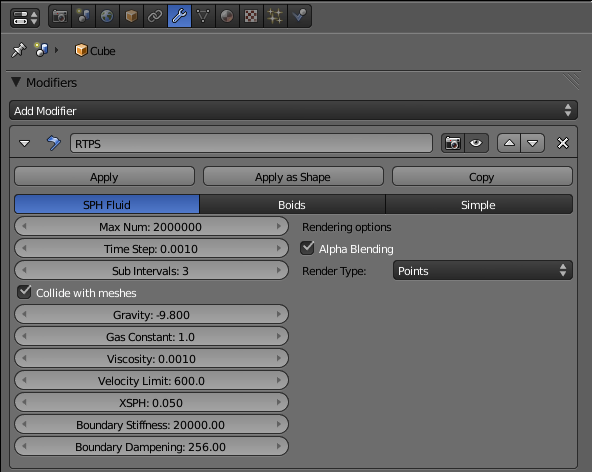
\includegraphics[scale=0.6]{figures/ui_mod.png}
        \caption{ RTPS Modifier UI panel }
		\label{fig:ui_mod}
\end{figure}


For this project the \verb|RTPS Modifier| was created.\cite{enjaCustomModifier} The
data stored in the modifier are the configurations and run-time options for the
RTPS library.  These options are exposed to the game designer in a panel and
displayed according to a Python script which calls the RNA API. The RNA code
specifies aspects of the user interface such as the minimum and maximum values
allowed for an input, or the options available in a drop-down menu. The
appearance of the user interface elements is automatically created using the
defaults provided by Blender, which are suitable for the current configuration.


\subsection{Apply}
The values from the User Interface are passed to the RTPS library when the
Modifier is Applied at the start of the game. The control flow is as follows,
the Game Engine iterates through all of the objects in the scene and if the
object has a Modifier the Modifier's apply routine is called. This logic is
extended to check explicitly for the \verb|RTPS Modifier|, and if present initialize
an RTPS instance.


The initialization involves passing in the values of the Modifier struct to the
RTPS settings instance as well as constructing a Domain object from the Axis
Aligned bounding box of the object which the Modifier is Applied to.

\subsection{Update}

The Update routine works similarly to the Apply routine with respect to control
flow. The Update routine is called for every frame of the game, rather than
only once at the start. In addtion to calling the update routine of the RTPS
instance, this is where most of the interaction between the Game Engine and the
library takes place.

\subsubsection{Collision}
Objects to be used for collision detection are dealt with in the update routine
by checking for a specific game property. If the boolean value of the
$collider$ property is true the faces of the object will be collected in a
vector and passed to the RTPS instance as Triangle objects. This does assume
that the mesh of the object is composed purely of Triangles. 
\begin{figure}[!htc]
 		\centering
		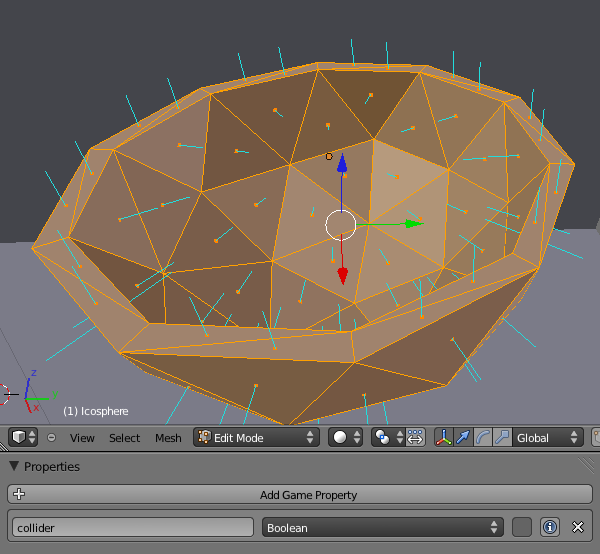
\includegraphics[scale=0.6]{figures/collision_ui.png}
        \caption{ Collision Object }
		\label{fig:collision_ui}
\end{figure}


\subsubsection{Emission}
Objects which emit particles are also handled in the Update routine. The
objects are detected and handled depending on which Game Properties are
present. Currently there are two types of emitters, Blob and Hose. A Blob
emitter will fill a user specified box with a user specified amount of
particles. The spacing of the particles is determined by the relation of the
particle radius to the domain size. This means that a user may attempt to fill
the volume with more particles than will fit, in which case only the number of
particles which fit will be emitted. If the user requests to emit more
particles than the maximum allowed, no particles will be emitted.
The Blob emitter is determined in blender by the presence of the $num$
property. Every frame, if the $num$ property is greater than zero, $num$
particles are emitted from the volume given by the Object's Axis Aligned
Bounding Box and the $num$ is set to zero. In this way it is possible to
provide interactive emissions of particles by using the Logic Bricks to change
the $num$ property during game play.
%screenshot

\begin{figure}[!htc]
 		\centering
		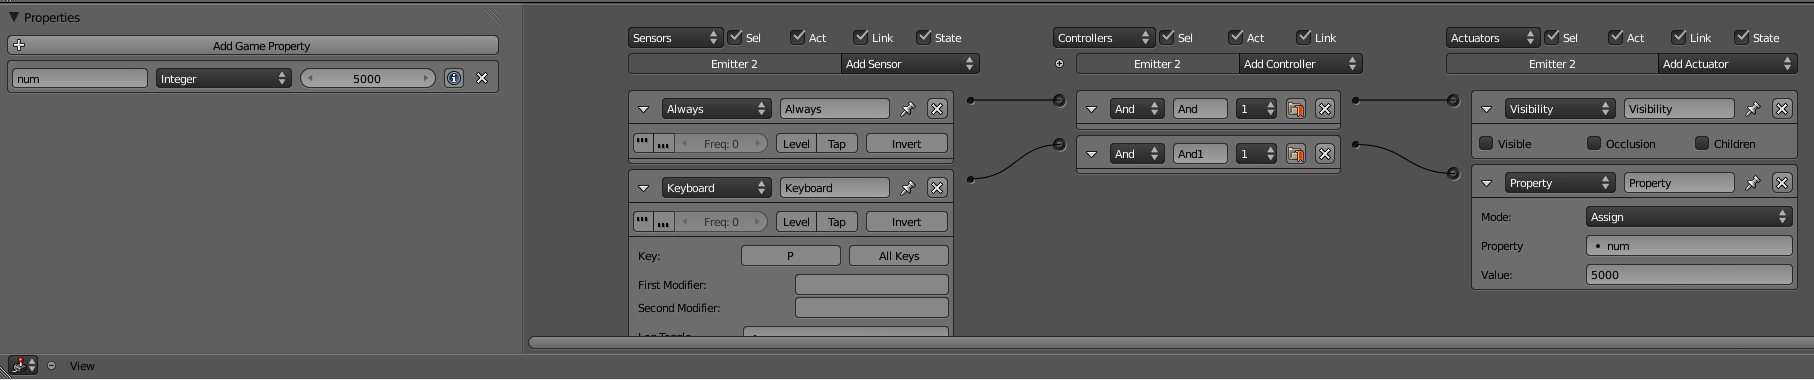
\includegraphics[scale=0.22]{figures/ui_emitter.png}
        \caption{ Logic panel showing Blob emitter }
		\label{fig:ui_emitter}
\end{figure}



The Hose emitter will spray a stream of particles in the direction and speed of
a user specified velocity vector. The radius of the nozzle is specified as a
multiple of the particle spacing. The Hose has a set number of particles it
will emit, and each frame a disc of particles is emitted at a rate proportional
to the time step and the velocity. The number of particles emitted each frame
is subtracted from the total number available to the Hose until there are no
more particles left, at which point the Hose will stop spraying. The positions
of the particles emitted in the disc are also slightly randomized (by one
particle spacing) along the velocity vector as well as along the plane of the
disc, giving a more natural depiction of spray.

A Hose is specified by the presence of the boolean $hose$ game property. The
value of the $hose$ property determines whether or not the Hose is activated.
The rest of the functionality for the Hose is controlled by the $num$, $radius$
and $speed$ properties. The $num$ property specifies the total amount of
particles available to the hose, the $speed$ property gives the initial
velocity of the particles emitted from the hose while the $radius$ determines
how wide the Hose is. The direction of the Hose is determined by the
orientation of the Y axis of the Hose Object.

\begin{figure}[!htc]
 		\centering
		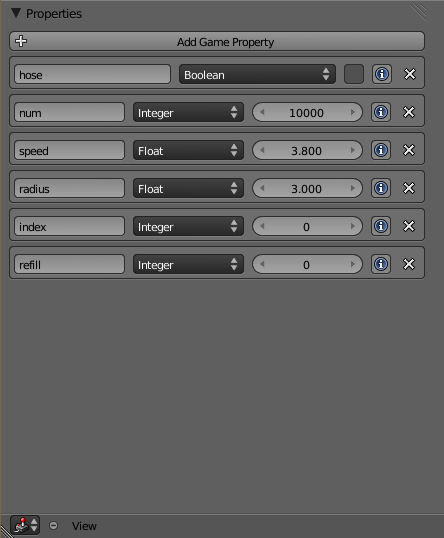
\includegraphics[scale=0.6]{figures/ui_hose.png}
        \caption{ Logic panel showing Hose emitter }
		\label{fig:ui_hose}
\end{figure}
\clearpage

\subsection{Orientation}
In Blender Objects are positioned in a Global coordinate system, with data
(such as vertices) specified in a Local coordinate system relative to the
Object's center. In the RTPS library particles are positioned in a coordinate
system relative to the Domain. In order for Blender and RTPS objects to
interact it is essential that objects can be represented in one of the two
coordinate systems. This is accomplished by using Blender's Global coordinate
system when passing information from Blender to RTPS. To use the Global
coordinate system for an Object, one multiplies a given local coordinate by the
Global Rotation and Transformation matrices maintained by the Game Engine for
the Object. This is done for the Domain, as well as Collider and Emitter
Objects, making all spatial coordinates in RTPS the Blender Global coordinates.

%screenshot
\subsection{Render}
Rendering of the RTPS particles in the Blender Game Engine is accomplished by
taking control of the way the Object with the \verb|RTPS Modifier| is displayed. The
Game Engine manages a list of all Objects to be rendered and calls various
OpenGL rasterization routines depending on properties and materials of the
Object. In order to render the RTPS particles the $render$ method of the RTPS
instance must be called. In the Game Engine rasterization code a conditional
statement was added to check for the presence of the \verb|RTPS Modifier|, and if
present the normal rendering is bypassed and the $render$ routine of the RTPS
instance is called instead.

\subsection{Files}
For a complete list of Blender source files modified by the project please
refer to Appendix \ref{appendix:modified} 

